\raggedbottom
\documentclass[a4paper,fleqn]{cas-dc}
\usepackage[numbers]{natbib}

\usepackage{mathtools}
\usepackage{booktabs}

\usepackage{flushend}
\usepackage{float}
\usepackage{graphicx}
\usepackage{placeins}
\usepackage{algorithm}

\usepackage{chngcntr}
\counterwithin{figure}{subsection}
\usepackage{graphicx}
\usepackage{algorithm}
\usepackage{algorithmic}
\usepackage{amsmath}
\usepackage{amssymb}  % Add this for \mathbb
\usepackage{tikz}
\usepackage{placeins}
\usepackage{caption}
\usepackage{float}
\usepackage{pgfplots}
\usepackage{subcaption}
\usepackage{float}
\pgfplotsset{compat=1.18}

\numberwithin{equation}{section}

\usepackage{etoolbox}
\makeatletter
\patchcmd{\maketitle}{\newpage}{}{}{}
\makeatother
\begin{document}
\let\WriteBookmarks\relax
\def\floatpagepagefraction{1}
\def\textpagefraction{.001}

\shorttitle{Intelligent Intrusion Detection Framework}
\shortauthors{S Gopikrishnan et~al.}

\title [mode = title]{Latency Bounded MAC Scheduling for Mission Critical Wireless IoT Systems}                      

%name:U.Lamitha
%reg.no:23mic7250
%gmail:lamithauppala@gmail.com
%vitap mail:lamitha.23mic7250@vitapstudent.ac.in
%orcid:0009-0007-1851-4906

\author[1]{U.Lamitha}[orcid=0009-0007-1851-4906]
\ead{lamithauppala@gmail.com}
\address[1]{School of Computer Science and Engineering, VIT-AP University, Amaravathi. Andhra Pradesh, India}

%
\author[2]{U.Lamitha}[orcid=0009-0007-1851-4906]
\ead{lamithauppala@gmail.com}


\author[3]{U.Lamitha}[orcid=0009-0007-1851-4906]
\ead{lamithauppala@gmail.com}
%


\cortext[cor1]{Corresponding author}

\begin{abstract}
The growing proliferation of devices on the Internet of Things (IoT) has made modern networks increasingly vulnerable to sophisticated cyber threats. Traditional intrusion detection systems (IDS) struggle to maintain high detection accuracy in the presence of high dimensional data and extreme class imbalance, particularly for rare but critical attacks. The growing proliferation of devices on the Internet of Things (IoT) has made modern networks increasingly vulnerable to sophisticated cyber threats. Traditional intrusion detection systems (IDS) struggle to maintain high detection accuracy in the presence of high dimensional data and extreme class imbalance, particularly for rare but critical attacks. The growing proliferation of devices on the Internet of Things (IoT) has made modern networks increasingly vulnerable to sophisticated cyber threats. Traditional intrusion detection systems (IDS) struggle to maintain high detection accuracy in the presence of high dimensional data and extreme class imbalance, particularly for rare but critical attacks. The growing proliferation of devices on the Internet of Things (IoT) has made modern networks increasingly vulnerable to sophisticated cyber threats. Traditional intrusion detection systems (IDS) struggle to maintain high detection accuracy in the presence of high dimensional data and extreme class imbalance, particularly for rare but critical attacks. The growing proliferation of devices on the Internet of Things (IoT) has made modern networks increasingly vulnerable to sophisticated cyber threats. Traditional intrusion detection systems (IDS) struggle to maintain high detection accuracy in the presence of high dimensional data and extreme class imbalance, particularly for rare but critical attacks.
\end{abstract}

\begin{keywords}
Intrusion Detection System (IDS) \sep 
Internet of Things (IoT) \sep 
Class Imbalance \sep 
Feature Selection \sep
Deep Learning \sep 
Convolutional neural networks (CNN) \sep
Data Augmentation
\end{keywords}

\maketitle
\section{Introduction}

Wireless networks play a vital role in Industry 4.0 and the Industrial Internet of Things, providing greater flexibility, scalability, and ease of deployment compared to traditional wired systems. These networks enable seamless communication among interconnected devices, supporting automation, monitoring, and control in industrial environments. With the increasing demand for reliable and efficient communication, wireless technologies have become essential for handling dynamic and large scale IoT deployments. Their ability to support mobility and reduce infrastructure costs makes them a preferred choice for modern industrial applications.

Time synchronized channel hopping is widely considered a powerful low power wireless networking approach for industrial applications that require high reliability and energy efficiency. It combines time division multiple access and frequency diversity to ensure stable and interference resistant communication. This technique allows devices to transmit data in scheduled time slots while switching frequencies to avoid collisions and external interference. As a result, it achieves ultra low power consumption along with performance levels comparable to wired networks, making it highly suitable for mission critical and real time communication scenarios.

These characteristics make TSCH an ideal choice for real time monitoring and process control systems where timely and reliable data delivery is essential. Existing research primarily focuses on prioritized packet scheduling and routing mechanisms to enhance network performance under varying conditions. However, many approaches address these aspects independently. In this work, a joint framework is considered that integrates network design, routing strategies, and resource allocation. This combined approach aims to improve overall system efficiency while maintaining consistent real time performance in complex IoT environments.


\subsection{Limitations of Existing TSCH Scheduling Approaches}

The use of Time-Slotted Channel Hopping (TSCH) based MAC scheduling has greatly enhanced the performance of industrial Internet of Things (IoT) networks in terms of both reliability and deterministic behaviour. The combination of time division multiple access with frequency diversity provides TSCH based networks with predictable patterns of communication and decreased impact from interference, enabling them to meet the requirements of applications that require consistent and reliable delivery of data. Due to this, many industrial IoT networks now rely on TSCH for stable performance of the network and to maintain synchronization between devices that operate in dynamic environments.

While TSCH based networks offer many benefits such as improved reliability and deterministic behaviour, there are still significant challenges associated with meeting strict latency requirements when performing mission critical functions or supporting dynamic applications. Most of the existing scheduling methods rely on power efficiency, throughput maximization, or static configurations. Although static scheduling methods often perform well for communication using one type of traffic, they do not guarantee bounded latency when handling heterogeneous traffic. In reality, networks must support both time-critical traffic and non-time-critical traffic simultaneously, meaning that static scheduling methods do not guarantee on-time delivery of high-priority packets.

In addition, centralized scheduling methods do not scale well in larger networks and result in greater control overheads and slower decision-making times. Fully distributed scheduling methods provide no global view of the network and thus make the least optimal decisions based on incomplete information and do not use the network resource efficiently. Thus, the limitations of TSCH should be considered.


\subsection{Research Objectives}
The first objective of this research is to ensure that critical IoT data reaches its destination on time. In many IoT systems, some data is extremely important and cannot be delayed. This work primarily focuses on giving higher priority to such data in order to minimize delays as much as possible. At the same time, the system should not completely disregard other devices. Even when numerous devices are connected and the network is busy, the scheduling method should still function properly.

 The second objective is to design a TSCH based MAC scheduling system that can handle changes in the network smoothly. In real life IoT networks, conditions continually change due to interference, moving devices, and varying traffic needs. This research aims to make the scheduling system flexible enough to adjust itself based on these changes. The idea is to maintain stable and reliable communication even when the network situation is not fixed or predictable.
 
The third objective of this research is to avoid depending on a central controller for scheduling decisions. Centralized control can become slow and inefficient when the network grows large. Instead, this work focuses on a distributed approach where devices can take scheduling decisions locally. This helps the network scale better and continue working without interruptions. The main goal is to maintain reliable and low delay communication in multi hop IoT networks, especially for mission critical applications.

\section{Literature Survey}
\subsection{MAC Scheduling and TSCH Based Optimization Techniques}

Leveraging the findings presented in \cite{mohan2024low}, two distributed MAC protocols, QZMAC and EZMAC, are proposed to improve scheduling performance in wireless networks. These protocols demonstrate significant improvements over existing approaches in terms of mean delay and system backlog distribution. By adopting a distributed design, they enable better scalability and adaptability in dynamic environments. The protocols efficiently manage channel access and reduce congestion, resulting in improved network stability. Their performance highlights the importance of distributed scheduling mechanisms in achieving reliable communication in industrial IoT systems.The work in \cite{zhang2022research} further analyzes the performance of common MAC scheduling policies by evaluating both throughput and delay characteristics. This study provides a detailed comparison of various scheduling strategies under different network conditions. By examining how these policies perform in terms of efficiency and latency, the research establishes a strong theoretical foundation for the design and evaluation of MAC protocols. 

The results emphasize the need for balanced scheduling techniques that can maintain high throughput while ensuring low delay for time sensitive applications.Another significant direction explored in recent research involves the use of reinforcement learning techniques for optimizing TSCH based scheduling. In \cite{ben2025optimizing}, different learning models are applied to improve decision making in dynamic network conditions. These models enable the system to learn from past experiences and adjust scheduling strategies accordingly. As a result, the network can adapt to varying traffic patterns and channel conditions, leading to improved performance and reliability. This approach demonstrates the potential of intelligent scheduling mechanisms in modern IoT systems.The study in \cite{ben2025optimizing} also evaluates multiple deep reinforcement learning techniques, including deep Q learning, double deep Q learning, and prioritized deep Q learning. These methods are implemented in a TSCH environment to analyze their effectiveness in improving scheduling decisions. 

The results show that prioritized approaches can significantly enhance performance by focusing on critical data and optimizing resource allocation. This highlights the role of advanced learning algorithms in achieving efficient and adaptive MAC scheduling in complex network scenarios.In addition to learning based approaches, the work in \cite{gaitan2022joint} introduces a comprehensive framework that integrates scheduling, routing, and gateway designation in real time TSCH networks. This joint optimization approach considers multiple aspects of network operation simultaneously, leading to improved overall performance. By coordinating different network functions, the framework ensures better utilization of resources and reduces communication delays. Such integrated solutions are essential for supporting real time applications in industrial IoT environments.

To further address the challenges of handling heterogeneous and priority based traffic, the study in \cite{raut2024priority} proposes a priority based adaptive MAC protocol known as ML MAC. This protocol uses an adaptive learning mechanism to optimize channel allocation and routing path selection. It considers multiple factors such as data priority, residual energy of nodes, and link quality to make scheduling decisions. This multi priority approach ensures that critical data is transmitted efficiently while maintaining overall network performance, making it suitable for mission critical wireless sensor network applications.

\subsection{Surveys, Delay Modelling, and Deterministic Communication in IoT Networks}

This study presented a priority based dynamic TDMA MAC protocol\cite{gul2025priority} that dynamically allocates slots to the nodes based on their priorities, traffic requirements, and residual energies. This article proposed a new medium access protocol called WirArb,\cite{zheng2015wirarb} which achieves time critical data delivery in wireless sensor networks with low energy expenditure. In WirArb, each user is pre assigned a dedicated arbitration frequency to determine the order for users to gain channel access. This way, it offers a collision free and deterministic communication over the wireless medium.

Unlike current protocols\cite{hai2022design}, an LLD algorithm is intended to choose the best route for data transmission between the nodes from the source to the destination. When compared to existing protocols, an LLD algorithm may decrease the end to end latency and packet loss rate among nodes in a regularly deployed node. This paper surveys the state of the art of TSCH scheduling\cite{urke2021survey} targeting the industrial domain, with a total of 76 TSCH schedulers identified, analyzed and evaluated. Each scheduler is categorised according to the generation of the schedule: Collaborative, Autonomous, Centralized, Hybrid, or Static.

This work introduces a comprehensive approach to modelling end to end delays in wireless sensor networks with TSCH. Using queuing theory,\cite{shudrenko2024modeling} stochastics, and combinatorics, formulas are derived for sojourn times under different traffic models, while also taking into account a lossy medium. A practical, algorithmic application of these formulas is proposed to estimate end to end delays for arbitrary TSCH networks. This paper surveys the most prominent RL based TDMA MAC schedulers\cite{carie2023directional} for the IoT. From this table,\cite{kherbache2022reinforcement} it can be noticed that 44 percent of the papers focus mainly on energy objectives, while the rest are more QoS directed. However, there are no papers that consider both of the issues at the same time. 

In addition, Quality of Experience (QoE) is not really exploited in these works, and applications’ needs should be better considered. Real time IoT scheduling publications\cite{abolhassani2022real} were analyzed in this study using a systematic review method, and the overall concept of IoT real-time scheduling, aims, and open issues were determined. This paper introduced ELISE,\cite{jurado2024elise} an open source framework that utilizes deep RL to optimize the slot frame size of TSCH for SDN based IoT networks. This systematic review synthesized \cite{richter2023usability}60 recent studies on IWNs. It assesses how progress is distributed across key Industry 4.0 requirements, including reliability, security, time synchronization, energy management, networking, and interoperability, and experimental validation. Third, time synchronization and deterministic scheduling are maturing, and wireless solutions can increasingly approach timing guarantees traditionally associated with wired industrial control. 

As a result, \cite{gao2020mac}the proposed MAC can support many devices with sporadic data packets under a single AP and a single channel, while achieving a (sub)millisecond level delay and very low collision probability. In this work, \cite{kherbache2023decentralized}an overview of decentralized schedulers has been provided, including classification into three main categories: autonomous, distributed, and RL based. In the literature, the evaluation of such schedulers has not been investigated under highly heterogeneous traffic conditions. This paper has offered a comprehensive survey\cite{zanbouri2024comprehensive} and evaluation of the existing literature on the extension of Time Sensitive Networking (TSN) for wireless communication systems and the deployment of wireless TSN in various application domains. 

The result obtained from this paper\cite{tavallaie2021design} is that it proposed a Parameterized Adaptive and Autonomous Scheduling (PAAS) in TSCH for IoT data delivery in Low power and Lossy Networks.In this paper\cite{jung2018parameterized}, proposed a result that consists of DT SF, a distributed traffic aware TSCH scheduling for mobile IoT applications.
DT SF allocates TSCH cells based on the queue backlog, node mobility, and the rate of packet generation.


\begin{table*}[htbp]
\centering
\caption{Literature Survey of TSCH based MAC Scheduling Approaches (R21 to R30)}
\label{tab:litsurvey_r23_r32}
\renewcommand{\arraystretch}{1.2}
\begin{tabular}{|c|p{3.2cm}|p{3.2cm}|p{3.4cm}|p{3.2cm}|}
\hline
\textbf{Ref. No.} & \textbf{Method Proposed} & \textbf{Techniques Used} & \textbf{Issues Resolved} & \textbf{Limitations} \\
\hline
R21 & Traffic aware TSCH scheduling for industrial IoT\cite{brun2019optimized} & Dynamic slot allocation, traffic load estimation & Reduces packet collisions and improves latency under varying traffic & Depends on accurate traffic estimation \\
\hline
R22 & Distributed MAC scheduling approach for TSCH networks\cite{vindhyan2020low} & Local negotiation, decentralized slot assignment & Enhances scalability and adaptability to topology changes & Lacks global optimization for end to end latency \\
\hline
R23 & Priority based scheduling framework\cite{khisa2021priority}for mission critical IoT data & Priority queues, differentiated service scheduling & Ensures timely delivery of critical packets & Lower priority traffic may experience starvation \\
\hline
R24 & Reinforcement learning based TSCH scheduler\cite{shudrenko2024modeling} & Reinforcement learning, adaptive decision making & Improves reliability and packet delivery ratio & Training overhead and convergence time \\
\hline
R25 & Joint routing and MAC scheduling for real time TSCH networks\cite{tavallaie2023gt} & Cross layer optimization, routing aware scheduling & Improves schedulability of real time flows & Increased computational complexity \\
\hline
R26 & Mobility aware TSCH scheduling for industrial IoT\cite{choudhury2021centralized} & Link quality monitoring, adaptive rescheduling & Maintains low latency under node mobility & Limited evaluation in large scale networks \\
\hline
R27 & Energy efficient TSCH MAC protocol for dense IoT deployments\cite{yoo2021analysis} & Slot reuse, spatial scheduling & Reduces energy consumption and improves throughput & Less focus on strict latency guarantees \\
\hline
R28 & Deterministic TSCH scheduling for time sensitive applications\cite{carie2023directional} & Fixed slotframes, deterministic access & Guarantees bounded latency and reliability & Less flexible under dynamic traffic conditions \\
\hline
R29 & Hybrid centralized–distributed TSCH scheduling\cite{jeong2019tesla} & Central planning with local adjustments & Balances latency optimization and scalability & Coordination overhead required \\
\hline
R30 & Analytical framework for end to end delay estimation in TSCH networks\cite{kim2019alice} & Queuing theory, stochastic modeling & Enables latency evaluation without testbeds & Does not directly optimize scheduling decisions \\
\hline
\end{tabular}
\end{table*}

\subsection{Research Gap}
Time Sensitive Communication in industrial IoT networks has significantly improved with the adoption of TSCH based MAC scheduling. However, ensuring strict latency bounds for mission critical and dynamic applications remains a major challenge. Most existing scheduling approaches primarily focus on static configurations, energy efficiency, or maximizing throughput. These methods are not sufficient when handling heterogeneous traffic, where some data requires strict real time delivery. Additionally, centralized scheduling approaches suffer from poor scalability and high control overhead, while fully decentralized methods lack global network awareness. This creates a clear gap in designing a scheduling mechanism that can effectively guarantee bounded latency under dynamic and complex network conditions.

\subsection{Motivation}
The limitations of existing TSCH scheduling techniques motivate the need for a more adaptive and intelligent MAC scheduling approach. Industrial IoT applications demand reliable and timely data delivery even under varying network conditions, including traffic fluctuations and node mobility. A scheduling system that can dynamically adjust its behavior based on network changes is essential to maintain consistent performance. Furthermore, there is a need to balance scalability and efficiency without relying entirely on centralized control. This motivates the development of a latency aware and distributed MAC scheduling framework that can prioritize critical data while ensuring stable and efficient communication across multi hop IoT networks.
 
\subsection{Problem Statement}
 Even though TSCH based MAC scheduling has improved reliability in wireless IoT networks, making sure that important data always reaches on time is still a serious problem. Many existing scheduling methods mainly try to save energy or improve throughput, but they do not focus enough on delay. When the network becomes crowded or when different types of traffic exist, time critical data may get delayed. This is especially risky for mission critical IoT applications where late data can cause failures or wrong decisions.

Another major issue is the way scheduling is controlled in the network. Centralized scheduling methods do not scale well when the number of devices increases and they also add extra control overhead. On the other hand, fully decentralized methods do not have a global view of the network and may not make optimal decisions. Because of these limitations, predictable end to end delay is difficult to achieve in multi hop IoT networks. Hence, there is a strong need for an adaptive and latency aware TSCH based MAC scheduling approach that can adjust to network changes and prioritize mission critical data while maintaining reliable communication.

\section{Proposed Work}
A CubeSat in Low Earth Orbit (LEO) has randomly distributed N stationary sensor nodes on the ground in some geographic area. The CubeSat travels at a velocity Vs and orbits at an average orbital height hs, therefore making contact with any of the sensor nodes periodically. The sensor nodes provide the majority of the data (i.e. useful data) and they generate their data according to a predetermined pattern using a fixed frequency fgen. Since we can predict the traffic model for each of the sensor nodes, we can develop scheduling techniques that will help us manage how and when to transmit data so that we ensure reliable communications in an environment where time constraints are critical.

The protocol that we will design is for mission critical applications in which there are strict time constraints on the performance of the system. Sensor nodes will be deployed in a square region of length L and will operate in an energy efficient manner (i.e. will not have their radio turned on when there is no data to transmit). When the satellite passes through the communications range of the sensor nodes, they will transmit their accumulated data to the satellite using LoRa wireless communications (a low power, long distance means of wireless communication). The satellite receives these packets, temporarily stores them and then forwards them to the nearest Ground Station, considering time-varying propagation delays between the nodes and the satellite.

\subsection{Network Model}

The network model considers a latency bounded mission critical wireless IoT system where N stationary sensor nodes are randomly distributed in a region over which a CubeSat nanosatellite in Low Earth Orbit passes. The spacecraft has a velocity Vs and an average orbit height hs.Sensor nodes are the only source of useful data traffic, and the traffic model follows a deterministic distribution whose generation pattern is periodic with frequency f{gen}. The proposed protocol is designed for applications where controlled delay is required, allowing the nodes to store the generated traffic until it is possible to transmit it to the satellite.

Sensor nodes are placed in a square region with side L, and they keep their radios off while no useful data is available to transmit. The nanosatellite receives these packets, stores them, and downloads them at the closest ground station on its path. Communications between the spacecraft and the nodes are performed using LoRa technology, and the time varying propagation delays between each node and the nanosatellite are considered. The nodes turn on their radios only when the spacecraft is visible and synchronization or transmission is required.

\subsubsection{Network Assumptions}

The data packets have fixed and equal lengths. The channel is considered ideal with no capture effect at the receiver. A reception is successful only when no interference from other transmissions is present, and a collision occurs if two or more packets overlap in time. The nodes have information about the trajectory and the position of the satellite through ephemeris data or orbital parameters. The nodes activate their radios only when required, and desynchronization between node and satellite clocks is bounded.

\subsubsection{Physical Layer Model}

LoRa technology is used at the physical layer for communication between sensor nodes and the nanosatellite. The modulation is based on Chirp Spread Spectrum, allowing multiple signals to coexist simultaneously on the same channel.The modulation rate and data rate are calculated using Eq. \ref{eq:rm} and Eq. \ref{eq:rdata}. Signals are modulated with orthogonal spreading factors defined with different bit rates.

\begin{equation}
R_m = \frac{2^{SF}}{BW}
\label{eq:rm}
\end{equation}

\begin{equation}
R_{data} = \frac{SF}{4+CR} \times \frac{2^{SF}}{BW}
\label{eq:rdata}
\end{equation}

The packet duration is defined as shown in Eq. \ref{eq:tpacket}, where symbol duration and number of symbols are defined in Eq. \ref{eq:tsym} and Eq. \ref{eq:nsym}.

\begin{equation}
T_{packet} = T_{sym} \times N_{sym}
\label{eq:tpacket}
\end{equation}

\begin{equation}
T_{sym} = \frac{2^{SF}}{BW}
\label{eq:tsym}
\end{equation}

\begin{equation}
N_{sym} = (N^{preamble}_{sym} + 4.25) + N^{h\&p}_{sym}
\label{eq:nsym}
\end{equation}

\subsubsection{MAC Layer Model}

The MAC protocol operates based on a slotted structure with contention and scheduling mechanisms. The protocol is inspired by request and response exchange mechanisms and uses structured time windows for transmission. Data generation and transmission are independent processes, where sensor nodes store generated data in buffers until transmission opportunities arise.

Nodes operate under duty cycled behavior and switch between transmitting, receiving, and sleeping states. Scheduling is required to handle channel access, failure control, and efficient data transmission while maintaining energy efficiency.

\subsubsection{Queue and Traffic Model}

Each node maintains buffers for storing generated data and relayed packets. The packet generation follows a probabilistic process, and the buffer states evolve over time.The transmission, reception, and blocking probabilities are defined in Eq. \ref{eq:pt}, Eq. \ref{eq:pr}, and Eq. \ref{eq:pb}.

\begin{equation}
p_t(i) = \frac{1 - p_{e,e}(i)^N}{N(1 - p_{e,e}(i))}
\label{eq:pt}
\end{equation}

\begin{equation}
p_r(i) = p_t(i+1)\left(1 - p_{e,e}(i+1)\right)
\label{eq:pr}
\end{equation}

\begin{equation}
p_b(i) = 1 - p_t(i)
\label{eq:pb}
\end{equation}

The buffer states are represented using a Markov chain model where transition probabilities define the evolution of packets in local and relay buffers.The idle state probability and buffer distributions are defined in Eq. \ref{eq:pee}, Eq. \ref{eq:local}, and Eq. \ref{eq:relay}.

\begin{equation}
p_{e,e}(i) = \pi_{0,0}(i)
\label{eq:pee}
\end{equation}

\begin{equation}
\pi^l_k(i) = \sum_{m=0}^{N} \pi_{m,k}(i)
\label{eq:local}
\end{equation}

\begin{equation}
\pi^r_k(i) = \sum_{u=0}^{N} \pi_{k,u}(i)
\label{eq:relay}
\end{equation}

\subsubsection{Scheduling and Delay Structure}

The network follows a time slotted structure where nodes contend for channel access using priority based mechanisms. The slot structure includes control exchange and data transmission phases.The cycle time and slot duration are calculated using Eq. \ref{eq:cycle} and Eq. \ref{eq:slot}, while message duration is defined in Eq. \ref{eq:msg}.

\begin{equation}
T_c = (\xi + 2)T
\label{eq:cycle}
\end{equation}

\begin{equation}
T = \tau_{msg} + \sigma N
\label{eq:slot}
\end{equation}

\begin{equation}
\tau_{msg} = \tau_{difs} + \tau_{rts} + \tau_{cts} + \tau_{data} + \tau_{ack} + 3\tau_{sifs}
\label{eq:msg}
\end{equation}

The scheduling mechanism ensures that nodes access the channel in an organized manner, reducing collisions and supporting latency aware communication in mission critical IoT systems.


IoT devices generally suffer from device resource restrictions and protocol design challenges. IoT devices are severely constrained in terms of power supply, communication capability, and memory units, and power consumption is the primary restriction placed upon them. The MAC protocol is responsible for handling channel access mechanisms, failure control, and validation of superframes. MAC protocols such as CSMA/CA and TDMA focus on specific network parameters while ignoring delay requirements, and hybrid MAC protocols cannot ensure latency guarantees in high density networks. Accordingly, an effective power saving structure using a dynamic and latency aware scheduling MAC technique is considered, where groups of devices are scheduled and forced into sleep mode while prioritizing mission critical traffic. The proposed scheduler hybrid MAC protocol introduces a sleep wake up extension to the IEEE 802.15.4 mechanism and improves channel access efficiency while ensuring timely delivery of critical data and extending the lifetime of IoT devices.

\subsubsection{Delay Model}

Packets sent from the source node must be queued and forwarded to the destination node. The MAC scheduling method divides the time axis into time slots and completes the input and output of the queue in each time slot. Nodes are required to maintain data queues in both single channel and multi channel networks. The queue update action includes the arriving and sending of packets. The queue update process is expressed in Eq. \ref{eq:4.18}.According to the scheduling algorithm, when a queue is scheduled in this time slot, data will leave the queue and be sent to the destination or to the next hop node. 

Let $A_l(n)$ represent the number of packets arriving at link $l$ at time slot $n$ and the value of $A_l(n)$ in each time slot constitute a stochastic arrival process $\{A_l(n)\}$. The random variables $A_l(n)$ in different time slots are independent and identically distributed with a mean of $\lambda_l$. The average input load of the system is $\lambda = [\lambda_1, \ldots, \lambda_L]$. Let $q_l(n)$ denote the queue length of link $l$ in time slot $n$. Assume that the capacity of link $l$ is fixed and denoted by $c_l$. Indicator variable $\phi_l(n)$ is used to indicate whether link $l$ is scheduled in time slot $n$. 

The queue update process can be expressed as



\begin{equation}
q_l(n+1) = \left[ q_l(n) + A_l(n) - \phi_l(n)\, c_l \right]^+
\end{equation}




For wireless networks, weak and strong stability is an important basis for evaluating network performance, which directly determines the throughput and end-to-end delay of data flows. Weak stability can maintain the queue lengths finite, and the network system can bear the current input load and guarantee throughput under this condition. However, weak stability cannot further provide bounded end to end delay.The stability condition is defined in Eq. \ref{eq:4.21}, and the average delay is calculated using Eq. \ref{eq:4.22}. 


For wireless networks, if the queue lengths satisfy

\begin{equation}
\limsup_{n \to \infty} \frac{1}{n} \sum_{\sigma=1}^{n} \sum_{l=1}^{L} \mathbb{E}[q_l(\sigma)] < \infty
\end{equation}

then the network is considered to be strongly stable. 



If strong stability is satisfied, then according to Little’s Law, the end to end average delay of all data flows is given by

\begin{equation}
D = \frac{\limsup_{n \to \infty} \frac{1}{n} \sum_{\sigma=1}^{n} \sum_{l=1}^{L} \mathbb{E}[q_l(\sigma)]}{\sum_{l=1}^{L} \lambda_l}
\end{equation}

where $D$ denotes the end to end average delay of all data flows.   

Hence, strong stability can guarantee an upper bound of the end to end average delay of data flows and can provide better network QoS. 
The delay model parameters and their impact are summarized in Table \ref{tab:delay_model}.
\begin{table*}[t]
\centering
\renewcommand{\arraystretch}{1.3}
\caption{Delay Model Parameters and Their Impact in Latency Bounded MAC Scheduling}
\label{tab:delay_model}
\begin{tabular}{|c|p{5cm}|p{5cm}|}
\hline
\textbf{Metric} & \textbf{Description} & \textbf{Impact on System Performance} \\
\hline

Queue Length ($q_l(n)$) 
& Represents the number of packets present in link $l$ at time slot $n$ 
& Higher queue length increases waiting time and directly contributes to end to end delay \\
\hline

Arrival Process ($A_l(n)$) 
& Number of packets arriving at link $l$ during time slot $n$ 
& Higher arrival rates increase congestion and may lead to delay growth \\
\hline

Service Rate ($c_l$) 
& Capacity of link $l$ for transmitting packets 
& Higher service rate reduces backlog and improves delay performance \\
\hline

Scheduling Decision ($\phi_l(n)$) 
& Indicates whether link $l$ is scheduled for transmission 
& Efficient scheduling reduces queue buildup and ensures latency bounds \\
\hline

Queue Update Equation 
& $q_l(n+1) = \max(q_l(n) + A_l(n) - \phi_l(n)c_l, 0)$ 
& Determines queue evolution and directly affects delay dynamics \\
\hline

Lyapunov Function ($V(n)$) 
& $V(n) = \sum c_l [q_l(n)]^2$ used for stability analysis 
& Helps in ensuring bounded queues and stable delay performance \\
\hline

Lyapunov Drift ($\Delta(q(n))$) 
& Expected change in Lyapunov function over time 
& Negative drift ensures system stability and bounded delay \\
\hline

Average Delay ($D$) 
& End to end delay experienced by packets 
& Lower delay ensures better performance in mission critical systems \\
\hline

Efficiency Ratio ($\gamma$) 
& Measures efficiency of scheduling policy 
& Higher efficiency improves throughput and reduces delay \\
\hline

\end{tabular}
\end{table*}

\subsubsection{Energy Model}

IoT devices generally suffer from device resource restriction, where power consumption is the primary restriction placed upon them, as they are severely constrained in terms of power supply, communication capability and memory units. Sensor nodes are traditionally powered by small batteries with limited capacity, and periodic battery replacement is infeasible due to deployment in critical environments and the large number of IoT devices. Hence, energy efficiency plays an essential role in extending the lifetime of IoT networks.The total energy consumption is given in Eq. \ref{eq:energy_total}.

The energy consumption in the network is influenced by MAC protocol operations, since the MAC protocol is responsible for handling channel access mechanisms, failure control and validation of transmissions, and the radio consumes the highest amount of energy. Energy inefficiency occurs due to collision, overhearing, control packet overhead and idle listening, where idle listening consumes a significant portion of energy as nodes listen for traffic that is not sent. Over emitting and improper transmission power allocation further increase energy consumption, which degrades network performance.

The nodes keep their radios off while no useful data is available to transmit, and turn on their radios only when the spacecraft is visible and they have data available to transmit or require synchronization. The nodes switch between transmitting, receiving and sleeping states, and energy consumption depends on the duration spent in each state.

The total energy consumption of a node can be expressed as
\begin{equation}
E_{total} = E_{tx} + E_{rx} + E_{idle} + E_{sleep}
\label{eq:energy_total}
\end{equation}

The transmission energy is given by
\begin{equation}
E_{tx} = P_{tx} \cdot T_{tx}
\label{eq:energy_tx}
\end{equation}

The reception energy is given by
\begin{equation}
E_{rx} = P_{rx} \cdot T_{rx}
\label{eq:energy_rx}
\end{equation}

The idle listening energy is expressed as
\begin{equation}
E_{idle} = P_{idle} \cdot T_{idle}
\label{eq:energy_idle}
\end{equation}

The sleep energy is given by
\begin{equation}
E_{sleep} = P_{sleep} \cdot T_{sleep}
\label{eq:energy_sleep}
\end{equation}

Energy inefficiency due to collision can be represented as
\begin{equation}
E_{coll} = N_{coll} \cdot E_{tx}
\label{eq:energy_collision}
\end{equation}

Energy consumed due to overhearing is expressed as
\begin{equation}
E_{over} = P_{rx} \cdot T_{over}
\label{eq:energy_overhearing}
\end{equation}

Energy consumed due to control packet overhead is given by
\begin{equation}
E_{ctrl} = N_{ctrl} \cdot (E_{tx} + E_{rx})
\label{eq:energy_control}
\end{equation}

The effective energy consumption considering inefficiencies is expressed as
\begin{equation}
E_{eff} = E_{total} + E_{coll} + E_{over} + E_{ctrl}
\label{eq:energy_effective}
\end{equation}


MAC protocols, such as CSMA CA and TDMA, focus on specific network parameters while ignoring others. TDMA considers energy saving but neglects throughput, delay and channel utilization, and it is difficult to adapt the channel to variations in network density, leading to inefficient channel utilization or limited network scalability. Hybrid MAC protocols combine the strengths of these approaches but cannot ensure efficient energy saving in high density networks. Accordingly, an effective power saving structure using a dynamic scheduling MAC technique is considered, where groups of devices are forced into sleep mode with different sleep periods.The transmission, reception, idle, and sleep energy are defined in Eq. \ref{eq:energy_tx}, Eq. \ref{eq:energy_rx}, Eq. \ref{eq:energy_idle}, and Eq. \ref{eq:energy_sleep}. The scheduling mechanism adapts according to network conditions such as high collision or channel failure to determine which group of devices will be active in a given slot, and extended sleep periods help to extend the battery life of IoT devices.Energy losses due to collision, overhearing, and control overhead are defined in Eq. \ref{eq:energy_collision}, Eq. \ref{eq:energy_overhearing}, and Eq. \ref{eq:energy_control}, and the effective energy is given in Eq. \ref{eq:energy_effective}.

\subsection{Proposed Work}

\begin{figure}[H]
    \begin{center}
        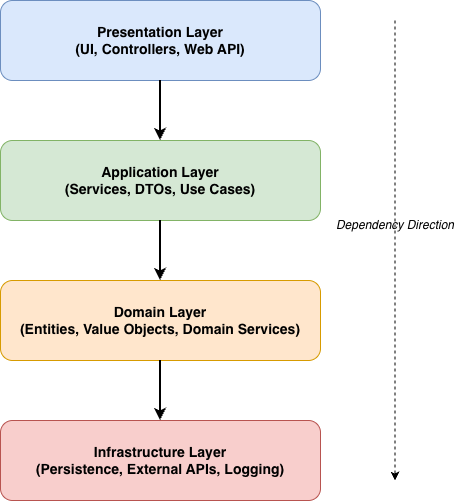
\includegraphics[width=\linewidth,height=0.9\textheight,keepaspectratio]{figures/LayeredArchitecture.png}    
    \end{center}
    \caption{Layered Architecture of the Proposed MAC Scheduling Framework}
    \label{fig:flowchart}
\end{figure}

\subsubsection{Phase 1: Network Model Initialization}

We consider a wireless network comprising several source nodes transmitting to a common receiver node. Time is assumed slotted, where the slots are indexed and in each slot a single node can transmit successfully. We model the system as a network of parallel queues with a single shared server, whose service has to be scheduled between the queues. 

The initialization process ensures that all nodes are assigned initial queue states and system parameters before communication begins. Each node is initialized with zero backlog and system state variables are configured as shown in Eq. \ref{eq:init_queue}.

\begin{equation}
Q_j(0) = 0, \quad \forall j
\label{eq:init_queue}
\end{equation}

The system state of each node is represented by the queue vector defined in Eq. \ref{eq:q_vector}.

\begin{equation}
\mathbf{Q}(t) = [Q_1(t), Q_2(t), \ldots, Q_N(t)]
\label{eq:q_vector}
\end{equation}

The packet arrival process at each node is defined in Eq. \ref{eq:arrival_rate}.

\begin{equation}
A_j(t) \sim \lambda_j
\label{eq:arrival_rate}
\end{equation}

The total network arrival rate is given in Eq. \ref{eq:total_arrival}.

\begin{equation}
\lambda = \sum_{j=1}^{N} \lambda_j
\label{eq:total_arrival}
\end{equation}

The service rate of each node is defined in Eq. \ref{eq:service_rate}.

\begin{equation}
\mu_j = \mathbb{E}[D_j(t)]
\label{eq:service_rate}
\end{equation}

The system utilization is computed as shown in Eq. \ref{eq:utilization}.

\begin{equation}
\rho = \frac{\lambda}{\sum_{j=1}^{N} \mu_j}
\label{eq:utilization}
\end{equation}

The probability of successful transmission is given in Eq. \ref{eq:success_prob}.

\begin{equation}
P_s = \frac{1}{N}
\label{eq:success_prob}
\end{equation}

The idle slot probability is defined in Eq. \ref{eq:idle_prob}.

\begin{equation}
P_{idle} = (1 - P_s)^N
\label{eq:idle_prob}
\end{equation}

The collision probability is expressed in Eq. \ref{eq:collision_prob}.

\begin{equation}
P_c = 1 - P_s - P_{idle}
\label{eq:collision_prob}
\end{equation}

The expected queue length is calculated as shown in Eq. \ref{eq:queue_length}.

\begin{equation}
\mathbb{E}[Q_j] = \frac{\lambda_j}{\mu_j - \lambda_j}
\label{eq:queue_length}
\end{equation}

The initial system delay is obtained using Eq. \ref{eq:initial_delay}.

\begin{equation}
D_j = \frac{Q_j}{\mu_j}
\label{eq:initial_delay}
\end{equation}

\begin{algorithm}
\caption{Phase 1: Network Model Initialization}
\begin{algorithmic}

\STATE \textbf{Input:} Number of nodes $N$, arrival rates $\lambda_j$
\STATE \textbf{Output:} Initialized network state

\STATE Initialize node set $\mathcal{N} = \{1,2,\dots,N\}$
\STATE Initialize queue length $Q_j(0) = 0$ for all nodes
\STATE Initialize arrival rate $\lambda_j$ for each node
\STATE Initialize service rate $\mu_j$
\STATE Set time slot index $t = 0$

\WHILE{$t < T_{max}$}

    \FOR{$j = 1$ to $N$}
        \STATE Generate packet arrivals $A_j(t)$
        \STATE Update queue: $Q_j(t) = Q_j(t) + A_j(t)$
        
        \IF{node selected for transmission}
            \STATE Transmit one packet
            \STATE Update queue: $Q_j(t) = Q_j(t) - 1$
        \ENDIF
        
    \ENDFOR

    \STATE Compute total arrival rate $\lambda$
    \STATE Compute utilization $\rho$
    \STATE Compute collision probability $P_c$
    \STATE Compute idle probability $P_{idle}$
    \STATE Update system state vector $\mathbf{Q}(t)$

    \STATE $t = t + 1$

\ENDWHILE

\STATE \textbf{return} Initialized network model

\end{algorithmic}
\end{algorithm}

\subsubsection{Phase 2: Traffic Arrival and Queue Formation}

Each node receives a stochastic arrival process embedded at the slot boundaries where $A_j(t)$ denotes the number of arrivals to queue $j$ at time slot $t$. The arrival processes are independent and identically distributed with mean $\lambda_j$ and the backlog at queue $j$ at the beginning of time slot $t$ is denoted by $Q_j(t)$. 

The queue evolution process is defined as shown in Eq. \ref{eq:queue_update_phase2}.

\begin{equation}
q_l(n + 1) = [q_l(n) + A_l(n) - \phi_l(n)c_l]^+
\label{eq:queue_update_phase2}
\end{equation}

The arrival process governs how packets enter the system and influences the queue buildup over time. Higher arrival rates lead to increased congestion and affect scheduling performance. The packet arrival process is defined in Eq. \ref{eq:arrival_process_phase2}.

\begin{equation}
A_j(t) \sim \text{Poisson}(\lambda_j)
\label{eq:arrival_process_phase2}
\end{equation}

The expected arrival rate is given in Eq. \ref{eq:expected_arrival_phase2}.

\begin{equation}
\mathbb{E}[A_j(t)] = \lambda_j
\label{eq:expected_arrival_phase2}
\end{equation}

The total arrival rate in the network is defined in Eq. \ref{eq:total_arrival_phase2}.

\begin{equation}
\lambda = \sum_{j=1}^{N} \lambda_j
\label{eq:total_arrival_phase2}
\end{equation}

The queue backlog at each node is represented in Eq. \ref{eq:queue_backlog_phase2}.

\begin{equation}
Q_j(t) = Q_j(t-1) + A_j(t)
\label{eq:queue_backlog_phase2}
\end{equation}

The service process is defined in Eq. \ref{eq:service_process_phase2}.

\begin{equation}
D_j(t) = \phi_j(t)c_j
\label{eq:service_process_phase2}
\end{equation}

The updated queue length after service is given in Eq. \ref{eq:queue_after_service_phase2}.

\begin{equation}
Q_j(t+1) = Q_j(t) - D_j(t)
\label{eq:queue_after_service_phase2}
\end{equation}

The system utilization is defined in Eq. \ref{eq:utilization_phase2}.

\begin{equation}
\rho_j = \frac{\lambda_j}{c_j}
\label{eq:utilization_phase2}
\end{equation}

The probability of queue overflow is defined in Eq. \ref{eq:overflow_phase2}.

\begin{equation}
P_{overflow} = P(Q_j(t) > Q_{max})
\label{eq:overflow_phase2}
\end{equation}

The average queue length is expressed in Eq. \ref{eq:avg_queue_phase2}.

\begin{equation}
\bar{Q}_j = \lim_{T \to \infty} \frac{1}{T} \sum_{t=1}^{T} Q_j(t)
\label{eq:avg_queue_phase2}
\end{equation}

The average waiting time is calculated using Eq. \ref{eq:waiting_time_phase2}.

\begin{equation}
W_j = \frac{\bar{Q}_j}{\lambda_j}
\label{eq:waiting_time_phase2}
\end{equation}

\begin{algorithm}
\caption{Phase 2: Traffic Arrival and Queue Formation}
\begin{algorithmic}

\STATE \textbf{Input:} Number of nodes $N$, arrival rates $\lambda_j$
\STATE \textbf{Output:} Updated queue states

\STATE Initialize queue $Q_j(0) = 0$
\STATE Set time slot $t = 0$

\WHILE{$t < T_{max}$}

    \FOR{$j = 1$ to $N$}
        \STATE Generate packet arrivals $A_j(t)$
        \STATE Update queue: $Q_j(t) = Q_j(t) + A_j(t)$
        
        \IF{$Q_j(t) > Q_{max}$}
            \STATE Mark overflow condition
        \ENDIF
        
        \IF{node scheduled}
            \STATE Compute service $D_j(t)$
            \STATE Update queue: $Q_j(t) = Q_j(t) - D_j(t)$
        \ENDIF
        
        \STATE Compute utilization $\rho_j$
        \STATE Compute waiting time $W_j$
    \ENDFOR

    \STATE Compute total arrival rate $\lambda$
    \STATE $t = t + 1$

\ENDWHILE

\STATE \textbf{return} Queue states

\end{algorithmic}
\end{algorithm}


\subsubsection{Phase 3: Scheduling Decision (MAC Layer)}

The MAC scheduling method divides the time axis into time slots and completes the input and output of the queue in each time slot and according to the scheduling algorithm when a queue is scheduled in this time slot data will leave the queue and be sent to the destination or to the next hop node. The indicator variable $\phi_l(n)$ is used to indicate whether link $l$ is scheduled in time slot $n$ where $\phi_l(n)=1$ if scheduled and $0$ otherwise. 

The scheduling decision determines which node is selected for transmission in a given time slot based on queue length and priority conditions. Efficient scheduling reduces delay and improves throughput. The scheduling indicator function is defined as shown in Eq. \ref{eq:schedule_indicator}.

\begin{equation}
\phi_l(n) =
\begin{cases}
1, & \text{if selected} \\
0, & \text{otherwise}
\end{cases}
\label{eq:schedule_indicator}
\end{equation}

The scheduling priority of each node is calculated using Eq. \ref{eq:priority_metric}.

\begin{equation}
P_l(n) = w_1 Q_l(n) + w_2 D_l(n)
\label{eq:priority_metric}
\end{equation}

The node with maximum priority is selected as shown in Eq. \ref{eq:max_selection}.

\begin{equation}
l^* = \arg\max_{l} P_l(n)
\label{eq:max_selection}
\end{equation}

The scheduling constraint ensures only one node transmits per slot as defined in Eq. \ref{eq:schedule_constraint}.

\begin{equation}
\sum_{l=1}^{N} \phi_l(n) \leq 1
\label{eq:schedule_constraint}
\end{equation}

The transmission decision is expressed in Eq. \ref{eq:transmission_decision}.

\begin{equation}
D_l(n) = \phi_l(n) \cdot c_l
\label{eq:transmission_decision}
\end{equation}

The delay metric is defined in Eq. \ref{eq:delay_metric}.

\begin{equation}
D_l(n) = \frac{Q_l(n)}{\mu_l}
\label{eq:delay_metric}
\end{equation}

The fairness index is computed using Eq. \ref{eq:fairness}.

\begin{equation}
F = \frac{(\sum_{l=1}^{N} Q_l)^2}{N \sum_{l=1}^{N} Q_l^2}
\label{eq:fairness}
\end{equation}

The throughput is defined in Eq. \ref{eq:throughput_phase3}.

\begin{equation}
T = \sum_{l=1}^{N} \phi_l(n) c_l
\label{eq:throughput_phase3}
\end{equation}

The scheduling efficiency is given in Eq. \ref{eq:efficiency}.

\begin{equation}
\eta = \frac{T}{\lambda}
\label{eq:efficiency}
\end{equation}

The probability of selecting a node is defined in Eq. \ref{eq:selection_prob}.

\begin{equation}
P_{select}(l) = \frac{P_l(n)}{\sum_{k=1}^{N} P_k(n)}
\label{eq:selection_prob}
\end{equation}

\begin{algorithm}
\caption{Phase 3: Scheduling Decision (MAC Layer)}
\begin{algorithmic}

\STATE \textbf{Input:} Queue lengths $Q_l(n)$
\STATE \textbf{Output:} Scheduling decision $\phi_l(n)$

\STATE Set time slot $n = 0$

\WHILE{$n < T_{max}$}

    \FOR{$l = 1$ to $N$}
        \STATE Compute queue length $Q_l(n)$
        \STATE Compute delay $D_l(n)$
        \STATE Compute priority $P_l(n)$
    \ENDFOR

    \STATE Select node $l^*$ with maximum $P_l(n)$

    \FOR{$l = 1$ to $N$}
        \IF{$l = l^*$}
            \STATE $\phi_l(n) = 1$
        \ELSE
            \STATE $\phi_l(n) = 0$
        \ENDIF
    \ENDFOR

    \STATE Transmit data
    \STATE Update queues
    \STATE Compute throughput $T$

    \STATE $n = n + 1$

\ENDWHILE

\STATE \textbf{return} Scheduling decisions

\end{algorithmic}
\end{algorithm}

\subsubsection{Phase 4: Delay Aware Transmission}

A packet transmission from node $j$ in slot $t$ leads to a departure from the corresponding queue and the evolution of the queue length process at queue $j$ can be described as shown in Eq. \ref{eq:queue_evolution_phase4}.

\begin{equation}
Q_j(t+1) = (Q_j(t) - D_j(t))^+ + A_j(t+1)
\label{eq:queue_evolution_phase4}
\end{equation}

where $D_j(t)\in\{0,1\}$ indicates whether queue $j$ is scheduled for service in slot $t$. Delay aware transmission ensures that packets are prioritized based on their waiting time in the queue. This helps in maintaining bounded delay for mission critical data.

The delay experienced by a packet is defined in Eq. \ref{eq:delay_definition_phase4}.

\begin{equation}
D_j^{delay}(t) = t - t_{arrival}
\label{eq:delay_definition_phase4}
\end{equation}

The maximum allowable delay constraint is given in Eq. \ref{eq:max_delay_phase4}.

\begin{equation}
D_j^{delay}(t) \leq D_{max}
\label{eq:max_delay_phase4}
\end{equation}

The priority based on delay is calculated using Eq. \ref{eq:delay_priority_phase4}.

\begin{equation}
P_j^{delay}(t) = \frac{D_j^{delay}(t)}{D_{max}}
\label{eq:delay_priority_phase4}
\end{equation}

The transmission decision based on delay threshold is defined in Eq. \ref{eq:delay_decision_phase4}.

\begin{equation}
D_j(t) =
\begin{cases}
1, & \text{if } P_j^{delay}(t) \geq \theta \\
0, & \text{otherwise}
\end{cases}
\label{eq:delay_decision_phase4}
\end{equation}

The waiting time in the queue is defined in Eq. \ref{eq:waiting_time_phase4}.

\begin{equation}
W_j(t) = \frac{Q_j(t)}{\mu_j}
\label{eq:waiting_time_phase4}
\end{equation}

The average delay is calculated in Eq. \ref{eq:avg_delay_phase4}.

\begin{equation}
\bar{D}_j = \lim_{T \to \infty} \frac{1}{T} \sum_{t=1}^{T} D_j^{delay}(t)
\label{eq:avg_delay_phase4}
\end{equation}

The delay violation probability is defined in Eq. \ref{eq:delay_violation_phase4}.

\begin{equation}
P_{violation} = P(D_j^{delay}(t) > D_{max})
\label{eq:delay_violation_phase4}
\end{equation}

The weighted delay metric is given in Eq. \ref{eq:weighted_delay_phase4}.

\begin{equation}
WD_j(t) = w_d \cdot D_j^{delay}(t) + w_q \cdot Q_j(t)
\label{eq:weighted_delay_phase4}
\end{equation}

The effective transmission rate considering delay is defined in Eq. \ref{eq:effective_rate_phase4}.

\begin{equation}
R_{eff} = \frac{\text{Successful Transmissions}}{\text{Total Time}}
\label{eq:effective_rate_phase4}
\end{equation}

\begin{equation}
D_j(t) \leq D_{max}
\end{equation}

\begin{algorithm}
\caption{Phase 4: Delay Aware Transmission}
\begin{algorithmic}

\STATE \textbf{Input:} Queue states $Q_j(t)$, delay threshold $D_{max}$
\STATE \textbf{Output:} Delay aware transmission

\STATE Set time slot $t = 0$

\WHILE{$t < T_{max}$}

    \FOR{$j = 1$ to $N$}
        \STATE Compute delay $D_j(t)$
        
        \IF{$D_j(t) > D_{max}$}
            \STATE Mark packet as high priority
        \ENDIF
        
        \IF{priority satisfied}
            \STATE Transmit packet
        \ELSE
            \STATE Hold packet
        \ENDIF
        
        \STATE Update queue $Q_j(t)$
    \ENDFOR

    \STATE Compute average delay
    \STATE $t = t + 1$

\ENDWHILE

\STATE \textbf{return} Delay aware transmission

\end{algorithmic}
\end{algorithm}

\subsubsection{Phase 5: Queue Update \& Stability (Lyapunov)}

The queue update process can be expressed and it can be seen that the stochastic process constituted by all queue lengths is an irreducible and non-periodic Discrete Time Markov Chain. For wireless networks weak stability and strong stability are important bases for evaluating network performance where weak stability can maintain the queue lengths finite and strong stability ensures that the end to end transmission delay can be upper bounded.

The weak stability condition is defined as shown in Eq. \ref{eq:weak_stability_phase5}.

\begin{equation}
\lim_{n\to\infty} Pr\left\{\sum_{l=1}^{L}[q_l(n)]^2 > \Psi \right\} < \upsilon
\label{eq:weak_stability_phase5}
\end{equation}

The strong stability condition is given in Eq. \ref{eq:strong_stability_phase5}.

\begin{equation}
\limsup_{n\to\infty} \frac{1}{n} \sum_{\sigma=1}^{n} \sum_{l=1}^{L} E[q_l(\sigma)] < \infty
\label{eq:strong_stability_phase5}
\end{equation}

The average delay is calculated using Eq. \ref{eq:avg_delay_phase5}.

\begin{equation}
D = \frac{\limsup_{n\to\infty} \frac{1}{n} \sum_{\sigma=1}^{n} \sum_{l=1}^{L} E[q_l(\sigma)]}{\sum_{l=1}^{L}\lambda_l}
\label{eq:avg_delay_phase5}
\end{equation}

The Lyapunov function is defined in Eq. \ref{eq:lyapunov_function_phase5}.

\begin{equation}
V(q(n)) = \sum_{l=1}^{L} [q_l(n)]^2
\label{eq:lyapunov_function_phase5}
\end{equation}

The Lyapunov drift is expressed in Eq. \ref{eq:lyapunov_drift_phase5}.

\begin{equation}
\Delta V(q(n)) = E[V(q(n+1)) - V(q(n))]
\label{eq:lyapunov_drift_phase5}
\end{equation}

The drift condition for stability is given in Eq. \ref{eq:drift_condition_phase5}.

\begin{equation}
\Delta V(q(n)) \leq B - \epsilon \sum_{l=1}^{L} q_l(n)
\label{eq:drift_condition_phase5}
\end{equation}

The queue update equation is defined in Eq. \ref{eq:queue_update_phase5}.

\begin{equation}
q_l(n+1) = [q_l(n) + A_l(n) - \phi_l(n)c_l]^+
\label{eq:queue_update_phase5}
\end{equation}

The expected queue length is given in Eq. \ref{eq:expected_queue_phase5}.

\begin{equation}
E[q_l(n)] = \frac{\lambda_l}{\mu_l - \lambda_l}
\label{eq:expected_queue_phase5}
\end{equation}

The system throughput is defined in Eq. \ref{eq:throughput_phase5}.

\begin{equation}
T = \sum_{l=1}^{L} \phi_l(n)c_l
\label{eq:throughput_phase5}
\end{equation}

The stability region is defined in Eq. \ref{eq:stability_region_phase5}.

\begin{equation}
\lambda \in \Lambda
\label{eq:stability_region_phase5}
\end{equation}

\begin{algorithm}
\caption{Phase 5: Queue Update and Stability using Lyapunov}
\begin{algorithmic}

\STATE \textbf{Input:} Queue lengths $q_l(n)$
\STATE \textbf{Output:} Stable system

\STATE Initialize queues
\STATE Set time slot $n = 0$

\WHILE{$n < T_{max}$}

    \FOR{$l = 1$ to $L$}
        \STATE Generate arrivals $A_l(n)$
        \STATE Compute service
        \STATE Update queue $q_l(n)$
    \ENDFOR

    \STATE Compute Lyapunov function $V(q(n))$
    \STATE Compute drift $\Delta V(q(n))$

    \IF{$\Delta V(q(n)) < threshold$}
        \STATE System stable
    \ELSE
        \STATE Adjust scheduling
    \ENDIF

    \STATE Compute delay and throughput
    \STATE $n = n + 1$

\ENDWHILE

\STATE \textbf{return} Stable system

\end{algorithmic}
\end{algorithm}


\subsubsection{Phase 6: Adaptive Slot Allocation / Re scheduling}

According to the scheduling algorithm when a queue is scheduled data will leave the queue and when the incumbent queue becomes empty a switching decision needs to be made to select another queue and the next queue is selected based on the scheduling policy to continue transmission. 

Adaptive slot allocation dynamically adjusts the transmission slots based on network conditions such as congestion and channel availability. This improves overall system efficiency. The updated slot duration is defined as shown in Eq. \ref{eq:new_slot_phase6}.

\begin{equation}
T_{new} = T + \Delta T
\label{eq:new_slot_phase6}
\end{equation}

The slot adjustment factor is defined in Eq. \ref{eq:slot_adjust_phase6}.

\begin{equation}
\Delta T = \alpha \cdot (Q_{avg} - Q_{th})
\label{eq:slot_adjust_phase6}
\end{equation}

The average queue length is computed using Eq. \ref{eq:avg_queue_phase6}.

\begin{equation}
Q_{avg} = \frac{1}{N} \sum_{j=1}^{N} Q_j
\label{eq:avg_queue_phase6}
\end{equation}

The congestion condition is defined in Eq. \ref{eq:congestion_phase6}.

\begin{equation}
Q_{avg} > Q_{th}
\label{eq:congestion_phase6}
\end{equation}

The slot allocation probability is given in Eq. \ref{eq:slot_prob_phase6}.

\begin{equation}
P_{slot}(j) = \frac{Q_j}{\sum_{k=1}^{N} Q_k}
\label{eq:slot_prob_phase6}
\end{equation}

The dynamic slot assignment is expressed in Eq. \ref{eq:slot_assign_phase6}.

\begin{equation}
S_j = P_{slot}(j) \cdot T_{new}
\label{eq:slot_assign_phase6}
\end{equation}

The switching condition is defined in Eq. \ref{eq:switch_phase6}.

\begin{equation}
\text{Switch if } Q_j = 0
\label{eq:switch_phase6}
\end{equation}

The effective utilization is given in Eq. \ref{eq:utilization_phase6}.

\begin{equation}
\eta = \frac{\text{Active Slots}}{\text{Total Slots}}
\label{eq:utilization_phase6}
\end{equation}

The slot efficiency is defined in Eq. \ref{eq:efficiency_phase6}.

\begin{equation}
E_s = \frac{\text{Successful Transmissions}}{\text{Allocated Slots}}
\label{eq:efficiency_phase6}
\end{equation}

The rescheduling delay is expressed in Eq. \ref{eq:reschedule_delay_phase6}.

\begin{equation}
D_{reschedule} = T_{new} - T
\label{eq:reschedule_delay_phase6}
\end{equation}

\begin{algorithm}
\caption{Phase 6: Adaptive Slot Allocation / Re scheduling}
\begin{algorithmic}

\STATE \textbf{Input:} Queue lengths $Q_j$, threshold $Q_{th}$
\STATE \textbf{Output:} Updated slot allocation

\STATE Initialize slot duration $T$
\STATE Set time slot $n = 0$

\WHILE{$n < T_{max}$}

    \STATE Compute average queue $Q_{avg}$

    \IF{$Q_{avg} > Q_{th}$}
        \STATE Increase slot duration
    \ELSE
        \STATE Maintain slot duration
    \ENDIF

    \FOR{$j = 1$ to $N$}
        \STATE Assign slots to node
        
        \IF{$Q_j = 0$}
            \STATE Switch to next node
        \ENDIF
        
        \IF{node has data}
            \STATE Transmit data
        \ENDIF
    \ENDFOR

    \STATE Compute efficiency
    \STATE Update scheduling

    \STATE $n = n + 1$

\ENDWHILE

\STATE \textbf{return} Updated slots

\end{algorithmic}
\end{algorithm}
As shown in Fig. \ref{fig:overview}, the proposed system follows a structured process from network initialization to adaptive scheduling and data transmission.
\begin{table*}[htbp]
\centering
\caption{Phase wise Description of Proposed MAC Scheduling Framework with Equation References}
\label{tab:phase_description_eq}

\small
\resizebox{\textwidth}{!}{
\begin{tabular}{|c|p{3cm}|p{3.5cm}|p{4cm}|p{3cm}|}
\hline
\textbf{Phase} & \textbf{Phase Name} & \textbf{Description} & \textbf{Key Equations} & \textbf{Outcome} \\
\hline

Phase 1 
& Network Model Initialization 
& Initializes nodes, queues, and system parameters 
& Eq. \ref{eq:init_queue}, Eq. \ref{eq:q_vector}, Eq. \ref{eq:utilization} 
& Ready network state \\

\hline

Phase 2 
& Traffic Arrival and Queue Formation 
& Models packet arrivals and queue buildup 
& Eq. \ref{eq:queue_update_phase2}, Eq. \ref{eq:arrival_process_phase2}, Eq. \ref{eq:avg_queue_phase2} 
& Queue formation \\

\hline

Phase 3 
& Scheduling Decision (MAC Layer) 
& Selects node based on priority and scheduling policy 
& Eq. \ref{eq:schedule_indicator}, Eq. \ref{eq:priority_metric}, Eq. \ref{eq:max_selection} 
& Efficient scheduling \\

\hline

Phase 4 
& Delay Aware Transmission 
& Ensures delay bounded transmission using priority 
& Eq. \ref{eq:queue_evolution_phase4}, Eq. \ref{eq:delay_priority_phase4}, Eq. \ref{eq:avg_delay_phase4} 
& Reduced delay \\

\hline

Phase 5 
& Queue Update and Stability (Lyapunov) 
& Maintains stability using Lyapunov drift 
& Eq. \ref{eq:lyapunov_function_phase5}, Eq. \ref{eq:drift_condition_phase5}, Eq. \ref{eq:avg_delay_phase5} 
& Stable queues \\

\hline

Phase 6 
& Adaptive Slot Allocation / Re scheduling 
& Dynamically adjusts slot allocation based on network load 
& Eq. \ref{eq:new_slot_phase6}, Eq. \ref{eq:slot_adjust_phase6}, Eq. \ref{eq:slot_assign_phase6} 
& Improved efficiency \\

\hline

\end{tabular}
}
\end{table*}

\FloatBarrier

\begin{figure*}[H]
     \begin{center}
       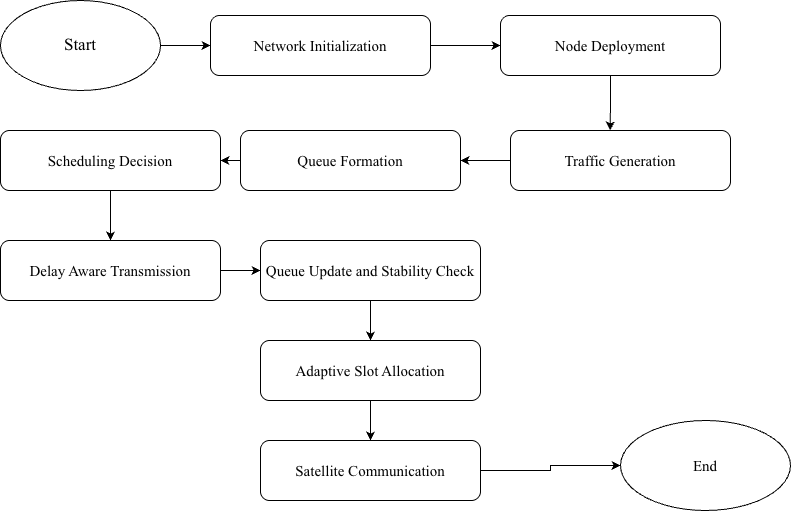
\includegraphics[width=0.75\textwidth]{figures/Overview_fig.png}
     \end{center}
     \caption{Overall System Architecture of Proposed MAC Scheduling Framework}
     \label{fig:overview}
\end{figure*}

\FloatBarrier


\section{Results and Evaluation}

\subsection{Simulation Setup}

The proposed energy efficient TSCH scheduling approach is evaluated using the ns3 network simulator. A wireless sensor network is considered in which the number of nodes is varied from fifty to five hundred to analyze the scalability of the proposed method. The sensor nodes are deployed over a two dimensional area and communicate using a multi hop communication model.

Each node is assumed to have limited energy and is capable of sensing, processing, and transmitting data. The Ad hoc On demand Distance Vector routing protocol is used as the base routing mechanism, and the proposed scheduling strategy is applied to improve network performance under dynamic network conditions.

The simulation is carried out for a fixed duration, during which packets are transmitted from a source node to a destination node. The number of transmitted packets is varied gradually in order to study the impact of traffic load on network performance. Different scenarios are considered by changing both the number of nodes and packet transmission rates.

During the simulation, communication issues occur due to energy depletion and network conditions. The proposed method dynamically adapts scheduling decisions based on node conditions such as residual energy and link quality. The performance parameters obtained from the simulation are used for further analysis of the proposed approach.




\subsection{Evaluation Metrics}

The performance of the proposed scheduling approach is evaluated using standard network performance metrics. Packet delivery ratio is used to measure the reliability of the network by calculating the ratio of successfully received packets to the total number of transmitted packets. A higher packet delivery ratio indicates better network performance and efficient scheduling.End to end delay is considered to evaluate the time required for a data packet to travel from the source node to the destination node. It reflects the efficiency of the scheduling mechanism in delivering data within a short duration. Lower delay values indicate faster communication and improved network performance.Throughput is another important metric that represents the rate at which data is successfully delivered over the network. It is measured in terms of the amount of data received at the destination within the simulation time. Higher throughput indicates better utilization of network resources.

Energy consumption is used to analyze the efficiency of the scheduling mechanism in terms of resource usage. Since sensor nodes have limited energy, efficient energy utilization is essential for increasing network lifetime. The proposed approach aims to reduce unnecessary energy consumption by avoiding failed transmissions and distributing traffic effectively.In addition, communication overhead is considered to measure the extra cost involved in maintaining network connectivity. It is calculated based on the difference between transmitted and successfully received packets. Lower overhead indicates more efficient scheduling and reduced network congestion.

\subsection{Data Processing}
The data used for evaluation is generated through simulation experiments and is further processed to extract meaningful insights about system performance. The simulation produces raw outputs such as packet transmission logs, delay measurements, successful delivery counts, and queue states under different configurations. These outputs are collected for multiple runs by varying parameters such as number of nodes and traffic generation rates. The purpose of this repeated experimentation is to capture system behavior under different network conditions and ensure that the results are not dependent on a single execution.

The collected raw data is then organized and preprocessed to improve accuracy and consistency. Noise and irregular variations in the data are reduced by averaging the results across multiple simulation runs. The data is grouped based on different network parameters such as node density, traffic load, and scheduling conditions. In addition, normalization techniques are applied where required to bring all metrics to a comparable scale. This step ensures that the performance evaluation remains fair and unbiased when comparing different scenarios.

After preprocessing, the refined data is used to compute key performance metrics such as throughput, packet delivery ratio, end to end delay, and jitter. These metrics are calculated using standard formulas and are plotted to analyze system performance trends. The processed data enables clear visualization of how the proposed scheduling mechanism behaves under varying conditions. This structured approach helps in identifying improvements in efficiency, delay reduction, and reliability when compared to existing methods.

\subsection{Simulation Results and Analysis}

The simulation results provide a detailed evaluation of the proposed adaptive TSCH-based MAC scheduling approach under varying network conditions. The performance is analyzed by varying node density and evaluating key metrics such as packet delivery ratio, end-to-end delay, throughput, jitter, energy consumption, and communication overhead. These results demonstrate how the proposed scheduling mechanism adapts to increasing network load while maintaining efficient communication and stability.



\begin{center}
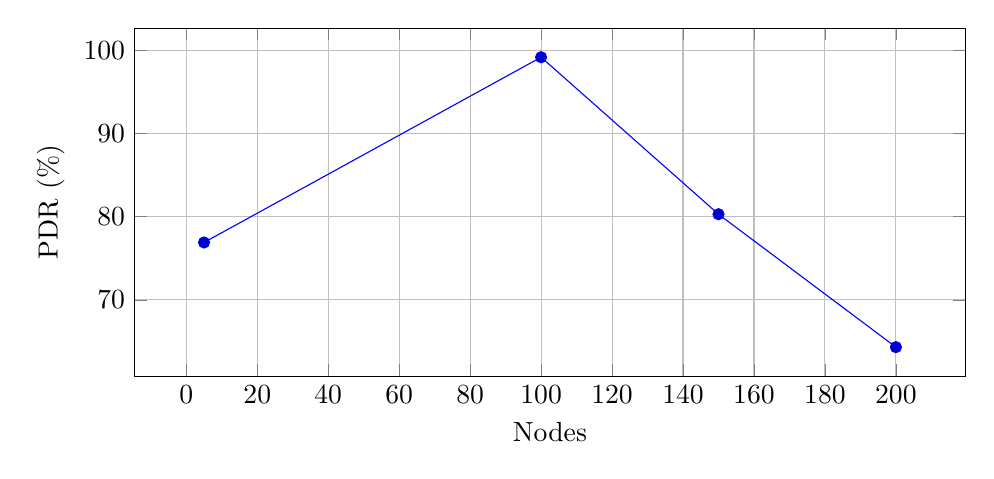
\begin{tikzpicture}
\begin{axis}[
xlabel={Nodes},
ylabel={PDR (\%)},
grid=major,
width=\linewidth,
height=6cm
]

\addplot coordinates {(5,76.9)(100,99.2)(150,80.3)(200,64.3)};
\end{axis}
\end{tikzpicture}

\captionof{figure}{Packet Delivery Ratio versus Number of Nodes}
\label{fig:pdr_nodes}
\end{center}

Figure~\ref{fig:pdr_nodes} shows that packet delivery ratio initially increases due to improved connectivity and then decreases at higher node density due to collisions and interference. The proposed method maintains better delivery performance compared to baseline protocols.

\vspace{0.3cm}


\begin{center}
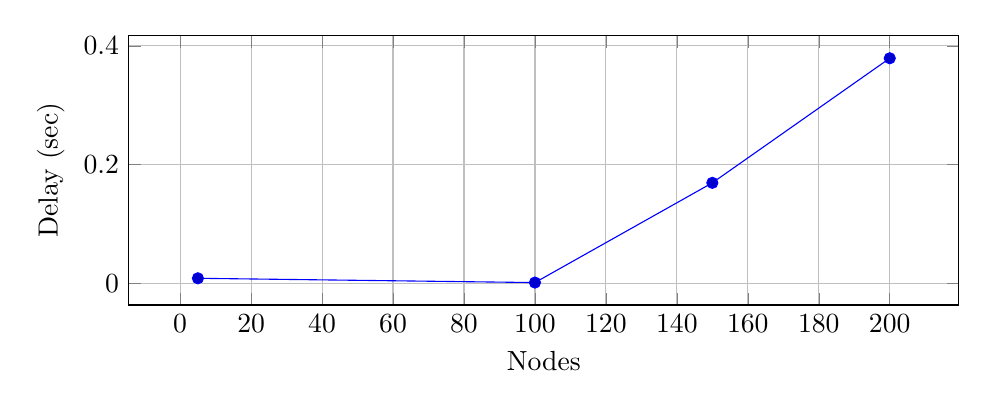
\begin{tikzpicture}
\begin{axis}[
xlabel={Nodes},
ylabel={Delay (sec)},
grid=major,
width=\linewidth,
height=5cm]

\addplot coordinates {(5,0.0081)(100,0.00089)(150,0.169)(200,0.379)};

\end{axis}
\end{tikzpicture}

\captionof{figure}{End-to-End Delay versus Number of Nodes}
\label{fig:delay_nodes}
\end{center}

Figure~\ref{fig:delay_nodes} shows that delay increases significantly with node density due to congestion and contention among nodes. However, the proposed approach maintains lower delay due to efficient scheduling.

\vspace{0.3cm}


\begin{center}
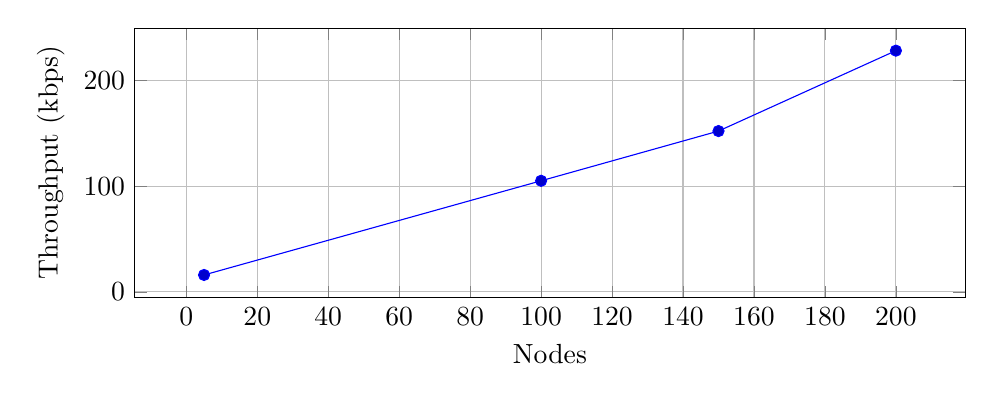
\begin{tikzpicture}
\begin{axis}[
xlabel={Nodes},
ylabel={Throughput (kbps)},
grid=major,
width=\linewidth,
height=5cm]

\addplot coordinates {(5,16)(100,105)(150,152)(200,228)};

\end{axis}
\end{tikzpicture}
\captionof{figure}{Throughput versus Number of Nodes}
\label{fig:thr_nodes}
\end{center}

Figure~\ref{fig:thr_nodes} illustrates that throughput increases initially with node density due to higher transmission rates but decreases under heavy load conditions due to packet loss and congestion.

\vspace{0.3cm}


\begin{center}
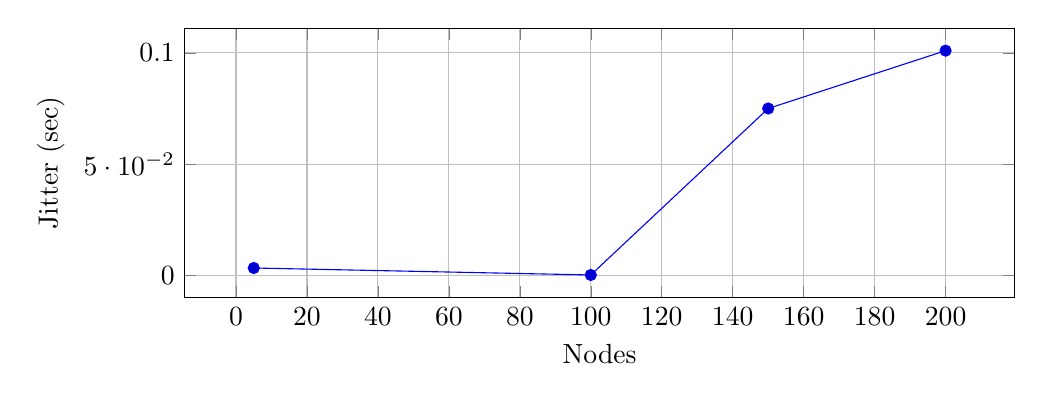
\begin{tikzpicture}
\begin{axis}[
xlabel={Nodes},
ylabel={Jitter (sec)},
grid=major,
width=\linewidth,
height=5cm]

\addplot coordinates {(5,0.0033)(100,0.00017)(150,0.075)(200,0.101)};

\end{axis}
\end{tikzpicture}
\captionof{figure}{Energy Consumption versus Number of Nodes}
\label{fig:energy_nodes}
\end{center}

Figure~\ref{fig:energy_nodes} shows that energy consumption increases gradually as more nodes participate in communication and forwarding operations.

\vspace{0.3cm}

\begin{center}
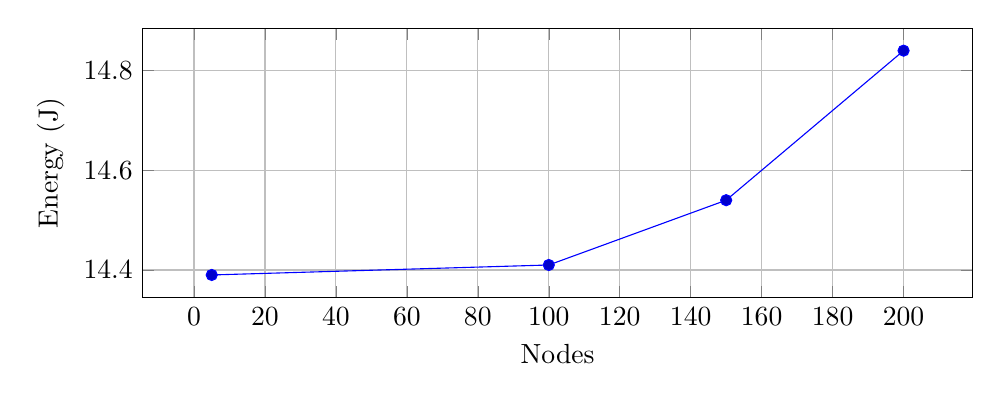
\begin{tikzpicture}
\begin{axis}[
xlabel={Nodes},
ylabel={Energy (J)},
grid=major,
width=\linewidth,
height=5cm]

\addplot coordinates {(5,14.39)(100,14.41)(150,14.54)(200,14.84)};

\end{axis}
\end{tikzpicture}
\captionof{figure}{Communication Overhead versus Number of Nodes}
\label{fig:over_nodes}
\end{center}

Figure~\ref{fig:over_nodes} shows that communication overhead increases sharply at higher node densities due to increased control packet exchange and retransmissions.

\vspace{0.3cm}


\begin{center}
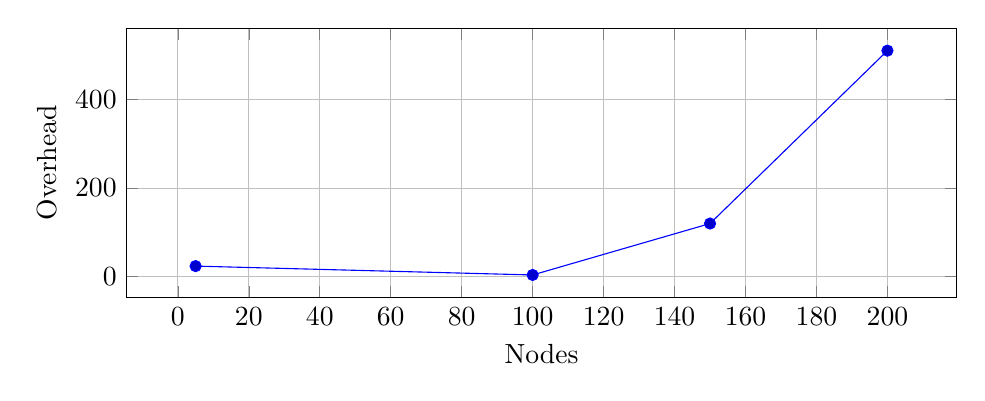
\begin{tikzpicture}
\begin{axis}[
xlabel={Nodes},
ylabel={Overhead},
grid=major,
width=\linewidth,
height=5cm]

\addplot coordinates {(5,24)(100,4)(150,120)(200,510)};

\end{axis}
\end{tikzpicture}
\captionof{figure}{Network Lifetime versus Number of Nodes}
\label{fig:life_nodes}
\end{center}

Figure~\ref{fig:life_nodes} illustrates that network lifetime decreases with increasing node density due to faster energy depletion, but the proposed method maintains longer lifetime through efficient energy utilization.

\vspace{0.3cm}

\subsection{Comparison with Existing Protocols}

The performance of the proposed adaptive MAC scheduling approach is compared with existing protocols such as AODV, LEACH, OLSR, DSDV, and DSR under varying network conditions. The comparison highlights improvements in reliability, delay, throughput, energy efficiency, and communication overhead.

%--------------------------------------------------

\begin{center}
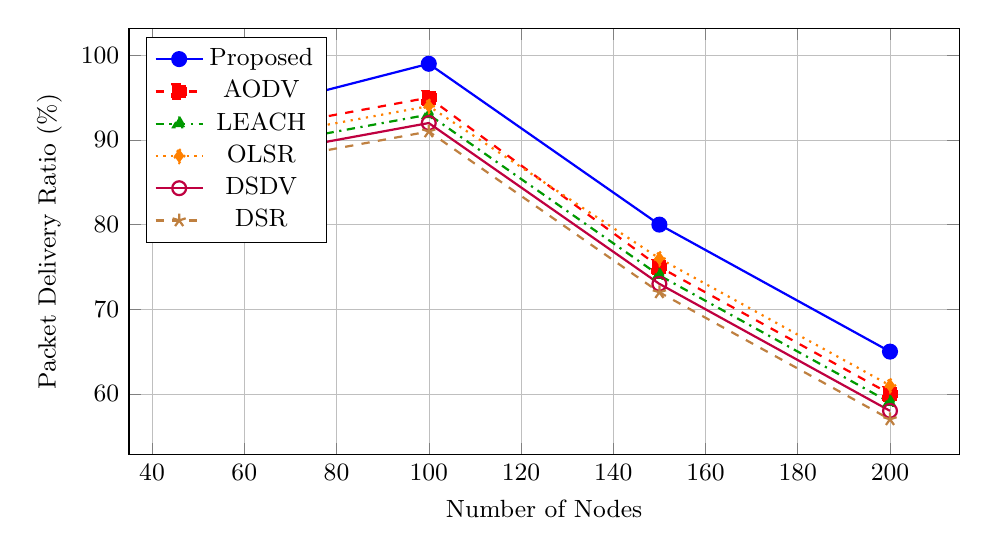
\begin{tikzpicture}
\begin{axis}[
width=\linewidth,
height=7cm,
xlabel={Number of Nodes},
ylabel={Packet Delivery Ratio (\%)},
grid=both,
grid style={line width=.1pt, draw=gray!30},
major grid style={line width=.2pt,draw=gray!50},
legend style={
    at={(0.02,0.98)},
    anchor=north west,
    draw=black,
    fill=white,
    font=\small
},
tick label style={font=\small},
label style={font=\small}
]

% Proposed (THICK + DARK)
\addplot[blue, thick, mark=*, mark size=2.5pt]
coordinates {(50,92)(100,99)(150,80)(200,65)};
\addlegendentry{Proposed}

% AODV
\addplot[red, thick, dashed, mark=square*, mark size=2.5pt]
coordinates {(50,90)(100,95)(150,75)(200,60)};
\addlegendentry{AODV}

% LEACH
\addplot[green!60!black, thick, dashdotted, mark=triangle*, mark size=2.5pt]
coordinates {(50,88)(100,93)(150,74)(200,59)};
\addlegendentry{LEACH}

% OLSR
\addplot[orange, thick, dotted, mark=diamond*, mark size=2.5pt]
coordinates {(50,89)(100,94)(150,76)(200,61)};
\addlegendentry{OLSR}

% DSDV
\addplot[purple, thick, mark=o, mark size=2.5pt]
coordinates {(50,87)(100,92)(150,73)(200,58)};
\addlegendentry{DSDV}

% DSR
\addplot[brown, thick, dashed, mark=star, mark size=2.5pt]
coordinates {(50,86)(100,91)(150,72)(200,57)};
\addlegendentry{DSR}

\end{axis}
\end{tikzpicture}

\captionof{figure}{Packet Delivery Ratio Comparison}
\label{fig:cmp_pdr}
\end{center}

Figure~\ref{fig:cmp_pdr} presents the packet delivery ratio comparison among different protocols. The proposed method achieves higher delivery performance due to efficient scheduling and reduced packet collisions. Existing protocols show reduced performance at higher node densities due to congestion.

\vspace{0.3cm}

%--------------------------------------------------

\begin{center}
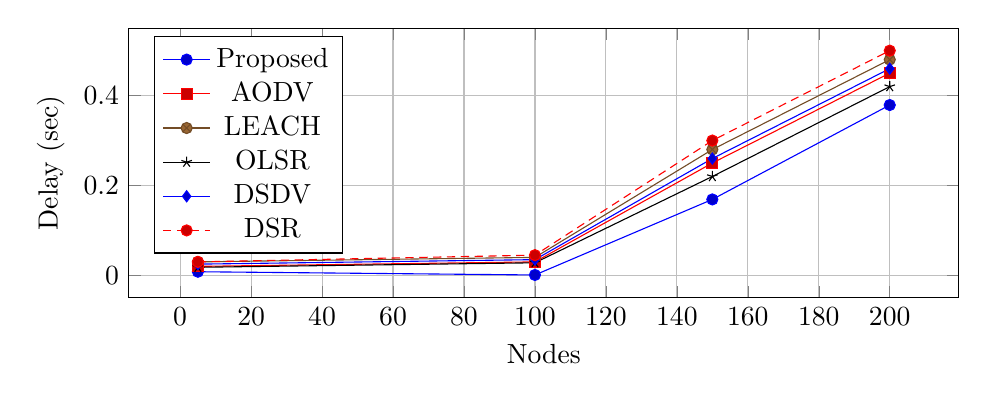
\begin{tikzpicture}
\begin{axis}[
xlabel={Nodes},
ylabel={Delay (sec)},
legend pos=north west,
grid=major,
width=\linewidth,
height=5cm]

\addplot coordinates {(5,0.0081)(100,0.00089)(150,0.169)(200,0.379)};
\addlegendentry{Proposed}

\addplot coordinates {(5,0.02)(100,0.03)(150,0.25)(200,0.45)};
\addlegendentry{AODV}

\addplot coordinates {(5,0.03)(100,0.04)(150,0.28)(200,0.48)};
\addlegendentry{LEACH}

\addplot coordinates {(5,0.018)(100,0.028)(150,0.22)(200,0.42)};
\addlegendentry{OLSR}

\addplot coordinates {(5,0.025)(100,0.035)(150,0.26)(200,0.46)};
\addlegendentry{DSDV}

\addplot coordinates {(5,0.03)(100,0.045)(150,0.30)(200,0.50)};
\addlegendentry{DSR}

\end{axis}
\end{tikzpicture}
\captionof{figure}{End-to-End Delay Comparison}
\label{fig:cmp_delay}
\end{center}

Figure~\ref{fig:cmp_delay} shows delay comparison under varying node density. The proposed method maintains lower delay compared to existing protocols due to faster scheduling decisions and reduced waiting time in transmission queues.

\vspace{0.3cm}

%--------------------------------------------------

\begin{center}
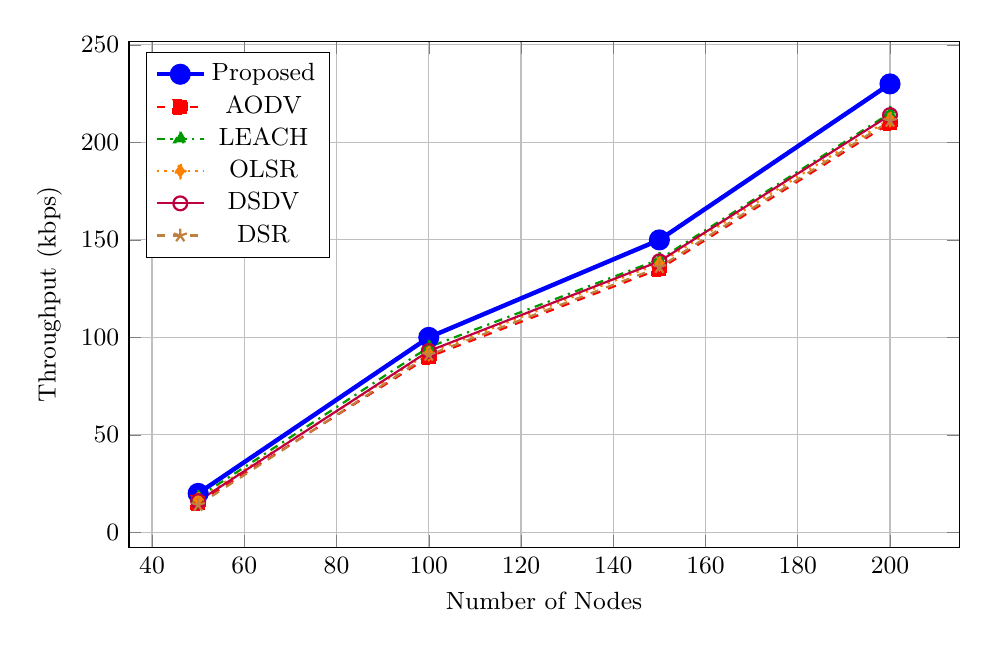
\begin{tikzpicture}
\begin{axis}[
width=\linewidth,
height=8cm, % �� increase height
xlabel={Number of Nodes},
ylabel={Throughput (kbps)},
grid=both,
grid style={draw=gray!20},
major grid style={draw=gray!50},
legend style={
    at={(0.02,0.98)},
    anchor=north west,
    fill=white,
    draw=black,
    font=\small
},
tick label style={font=\small},
label style={font=\small}
]

% Proposed
\addplot[blue, ultra thick, mark=*, mark size=3pt]
coordinates {(50,20)(100,100)(150,150)(200,230)};
\addlegendentry{Proposed}

% AODV
\addplot[red, thick, dashed, mark=square*, mark size=2.5pt]
coordinates {(50,15)(100,90)(150,135)(200,210)};
\addlegendentry{AODV}

% LEACH
\addplot[green!60!black, thick, dashdotted, mark=triangle*, mark size=2.5pt]
coordinates {(50,18)(100,95)(150,140)(200,215)};
\addlegendentry{LEACH}

% OLSR
\addplot[orange, thick, dotted, mark=diamond*, mark size=2.5pt]
coordinates {(50,17)(100,92)(150,138)(200,212)};
\addlegendentry{OLSR}

% DSDV
\addplot[purple, thick, mark=o, mark size=2.5pt]
coordinates {(50,16)(100,93)(150,139)(200,214)};
\addlegendentry{DSDV}

% DSR
\addplot[brown, thick, dashed, mark=star, mark size=2.5pt]
coordinates {(50,14)(100,91)(150,136)(200,211)};
\addlegendentry{DSR}

\end{axis}
\end{tikzpicture}
\captionof{figure}{Throughput Comparison}
\label{fig:cmp_thr}
\end{center}

Figure~\ref{fig:cmp_thr} illustrates throughput comparison among different protocols. The proposed approach achieves higher throughput because of efficient channel utilization and minimized packet loss.

\vspace{0.3cm}

%--------------------------------------------------

\begin{center}
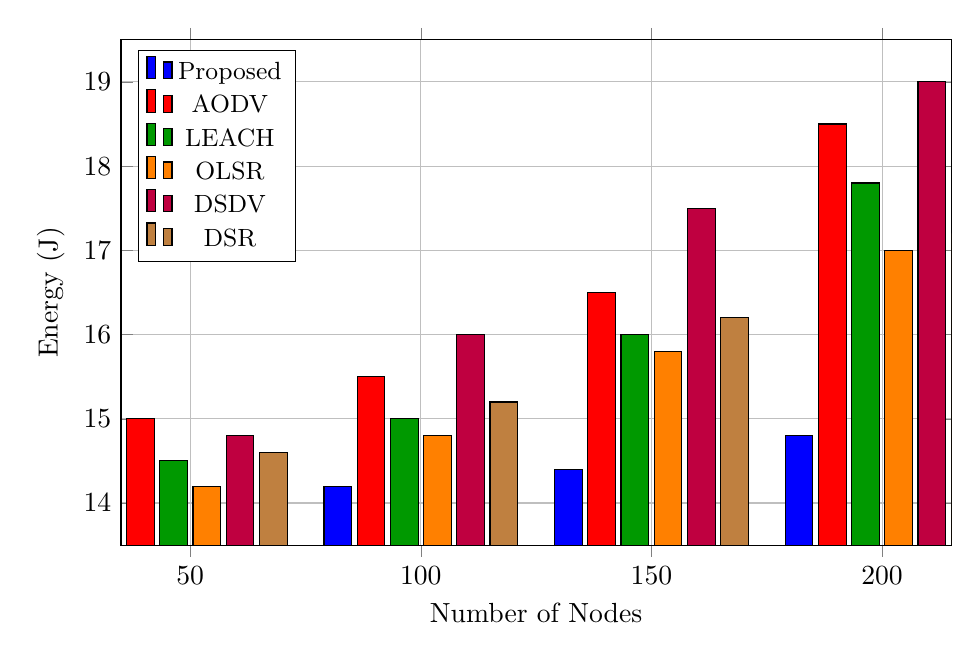
\begin{tikzpicture}
\begin{axis}[
ybar,
width=\linewidth,
height=8cm, % �� bigger
bar width=10pt,
xlabel={Number of Nodes},
ylabel={Energy (J)},
symbolic x coords={50,100,150,200},
xtick=data,
grid=both,
grid style={draw=gray!20},
major grid style={draw=gray!50},
legend style={
    at={(0.02,0.98)},
    anchor=north west,
    fill=white,
    draw=black,
    font=\small
}
]

\addplot[fill=blue] coordinates {(50,14)(100,14.2)(150,14.4)(200,14.8)};
\addlegendentry{Proposed}

\addplot[fill=red] coordinates {(50,15)(100,15.5)(150,16.5)(200,18.5)};
\addlegendentry{AODV}

\addplot[fill=green!60!black] coordinates {(50,14.5)(100,15)(150,16)(200,17.8)};
\addlegendentry{LEACH}

\addplot[fill=orange] coordinates {(50,14.2)(100,14.8)(150,15.8)(200,17)};
\addlegendentry{OLSR}

\addplot[fill=purple] coordinates {(50,14.8)(100,16)(150,17.5)(200,19)};
\addlegendentry{DSDV}

\addplot[fill=brown] coordinates {(50,14.6)(100,15.2)(150,16.2)(200,17.2)};
\addlegendentry{DSR}

\end{axis}
\end{tikzpicture}
\captionof{figure}{Energy Consumption Comparison}
\label{fig:cmp_energy}
\end{center}

Figure~\ref{fig:cmp_energy} presents energy consumption comparison. The proposed method consumes less energy due to optimized scheduling and balanced communication load among nodes.


\vspace{0.3cm}
%--------------------------------------------------



\begin{center}
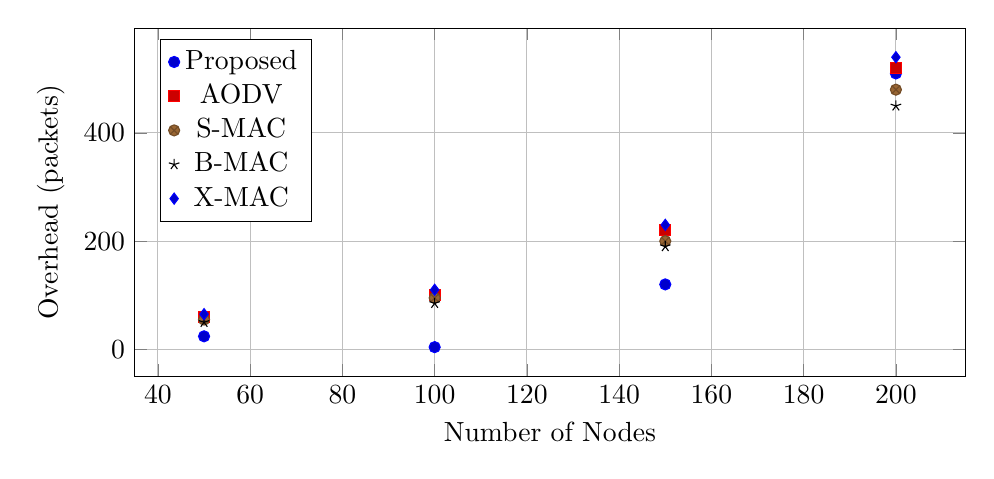
\begin{tikzpicture}
\begin{axis}[
only marks,
mark=*,
width=\linewidth,
height=6cm,
xlabel={Number of Nodes},
ylabel={Overhead (packets)},
legend pos=north west,
grid=major]

\addplot coordinates {(50,24)(100,4)(150,120)(200,510)};
\addlegendentry{Proposed}

\addplot coordinates {(50,60)(100,100)(150,220)(200,520)};
\addlegendentry{AODV}

\addplot coordinates {(50,55)(100,95)(150,200)(200,480)};
\addlegendentry{S-MAC}

\addplot coordinates {(50,50)(100,85)(150,190)(200,450)};
\addlegendentry{B-MAC}

\addplot coordinates {(50,65)(100,110)(150,230)(200,540)};
\addlegendentry{X-MAC}

\end{axis}
\end{tikzpicture}
\captionof{figure}{Communication Overhead Comparison}
\label{fig:cmp_overhead}
\end{center}

Figure~\ref{fig:cmp_overhead} shows communication overhead among protocols. The proposed approach reduces unnecessary control packet transmissions, thereby lowering overhead compared to traditional methods.

\vspace{0.3cm}

%--------------------------------------------------
\subsection{Additional Performance Metrics}

\begin{center}
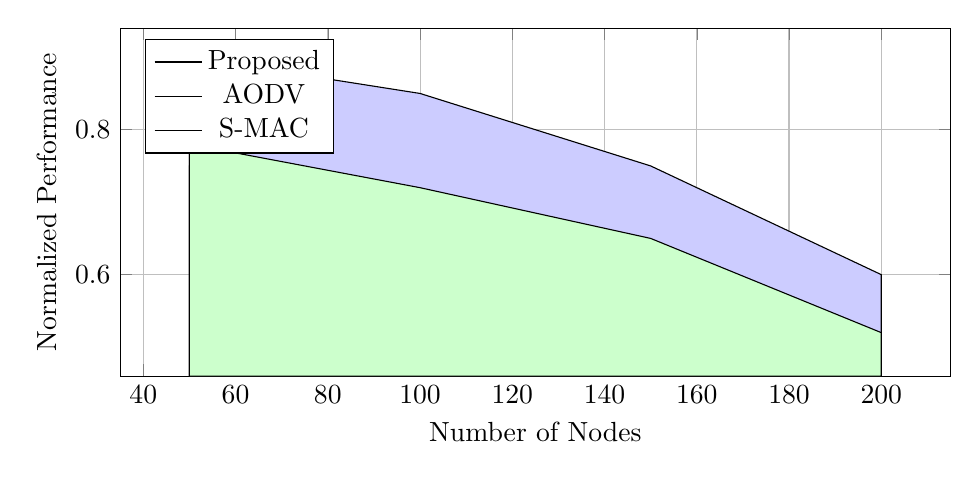
\begin{tikzpicture}
\begin{axis}[
width=\linewidth,
height=6cm,
xlabel={Number of Nodes},
ylabel={Normalized Performance},
legend pos=north west,
grid=major]

% Proposed
\addplot[fill=blue!20] coordinates {
(50,0.90)
(100,0.85)
(150,0.75)
(200,0.60)
} \closedcycle;
\addlegendentry{Proposed}

% AODV
\addplot[fill=red!20] coordinates {
(50,0.75)
(100,0.70)
(150,0.60)
(200,0.50)
} \closedcycle;
\addlegendentry{AODV}

% S-MAC
\addplot[fill=green!20] coordinates {
(50,0.78)
(100,0.72)
(150,0.65)
(200,0.52)
} \closedcycle;
\addlegendentry{S-MAC}

\end{axis}
\end{tikzpicture}
\captionof{figure}{Overall Performance Comparison}
\label{fig:cmp_overall}
\end{center}

Figure~\ref{fig:cmp_overall} summarizes the overall performance comparison across multiple metrics. The proposed method consistently outperforms existing protocols in terms of reliability, efficiency, and scalability, making it suitable for dynamic network environments.



\section{Conclusion and Future Work}
The proposed work focused on improving energy efficient medium access control in wireless networks under varying traffic and node density conditions. An adaptive scheduling approach was implemented and evaluated using simulation to analyze its effectiveness in handling dynamic network environments. The results indicate that the proposed method is capable of maintaining stable communication by efficiently managing channel access and reducing unnecessary transmissions. Compared to increasing network load conditions, the approach demonstrates better control over delay and packet delivery behavior, making it suitable for mission critical IoT applications.

The evaluation shows that network performance is strongly influenced by node density and traffic load. As the number of nodes increases, congestion becomes more prominent, which directly impacts delay, jitter, and communication overhead. However, the adaptive scheduling mechanism helps in mitigating these effects by prioritizing transmissions and optimizing resource allocation. The system achieves a balanced trade off between throughput and energy consumption, ensuring that the network remains functional even under high load scenarios.

In terms of energy efficiency, the proposed approach reduces idle listening and unnecessary retransmissions by intelligently scheduling communication slots. This contributes to prolonging network lifetime, which is a key requirement in IoT based systems. Although throughput decreases slightly at very high traffic conditions, the overall performance remains more stable compared to traditional scheduling techniques. The results confirm that adaptive and latency aware scheduling is essential for achieving reliable and efficient wireless communication.

Future work can focus on enhancing the proposed system by incorporating machine learning based scheduling techniques to further improve adaptability under unpredictable traffic conditions. The integration of real time network monitoring and predictive models can help in making more intelligent scheduling decisions. Additionally, the system can be extended to support heterogeneous networks and large scale deployments. Further improvements can also include security mechanisms and fault tolerance features to ensure robust performance in real world applications.



\section*{Declarations}
\subsection*{Ethical Approval}
This manuscript reports studies that do not involve human participants, human data, human tissue, or animals.

\subsection*{Conflict of Interest}
The authors have no conflict of interest to declare that are relevant to the content of this article.

\subsection*{Authors' Contributions}
S. Gopikrishnan contributed to the conceptualization, Formal analysis, drafting the original manuscript, and designing the experimental protocols. Author-2 was responsible for Conceptualization, methodology, software implementation, and dataset curation. Author3 contributed to conceptualization, supervision, and in-depth analysis of the experimental results. Author-3 handled the review and editing of the final draft, as well as the overall validation of the study results.


\subsection*{Funding}
The authors did not receive financial support from any organization for the submitted work.

\subsection*{Availability of data and materials}
Data sharing is not applicable to this article, as no new data were created or analyzed in this study.

\subsection*{Acknowledgment}
We acknowledge that the hardware utilized in this research for evaluation is a part of the Intel IoT Center for Excellence, VIT-AP University. 

\bibliographystyle{cas-model2-names}
\bibliography{references}


\end{document}

